\documentclass{article}
\usepackage[utf8]{inputenc}
\usepackage{graphicx}
\usepackage{siunitx}
\usepackage{xspace}
\usepackage{fancyhdr}
\pagestyle{fancy}
\fancyhf{}
\rfoot{\thepage}
\lfoot{}
\renewcommand{\headrulewidth}{0pt}

\title{\textbf{ Homework Assignment}}

\author{Concurrent and Distributed Systems}
\date{Student: Julia Florea

Calculatoare Engleza

Anul III, Grupa 3.2 A

Facultatea de Calculatoare, Automatică și Electronică}


\begin{document}
\maketitle
\vspace{10cm}
\textbf{ }
\textbf{}

\newpage






\section{Introduction}
\subsection{Problem statement}
Uncle John heard that selling organic eggs has become a great business nowadays. Therefore, he
decided to breed hens and create some farms for producing organic eggs. The hens lay eggs
which are picked up by his employees and sent to the farm headquarter.
Uncle John relies on you to help him implement the farm plan by using concurrency in Java.
\subsection{Instructions}
\begin{itemize}
\item \textbf{There are multiple farms:}  \\
-The hens are raised in farms. The number of farms is a random number between 2 and 5;\\ 
-Each farm is designed as a matrix with N x N where 100 $\le$ N $\le$ 500;\\ 
-Each farm has a list of hens;\\ 
-Every few seconds the farm monitoring system will request the position of the hens
inside the farm;\\ 
-There cannot be more than N / 2 hens for a farm.


\item \textbf{There are hens which produce eggs:}  \\
-The hens are spawning randomly in each farm at a random place, at a random time t,
where 500 $\le$ t $\le$ 1000 (milliseconds); \\ 
-Two hens cannot be in the same place;\\
\item \textbf{The hens lay eggs by:} \\ 
-Moving in one direction (left, right, up, down); \\ 
-When they reach the fence of the farm, they move in any other direction than the
fence; \\
-With each move, they lay an egg; \\
-If the hen is surrounded by other hens and cannot move in any direction, it stops for a
random time t, where 10 $\le$ t $\le$ 50 (milliseconds);\\
-Each time an egg is produced, the farm monitoring system informs the employees
about the position where the egg is located; \\
-After an egg is created, the hen needs to rest until it is able to produce another egg
(resting time is 30 milliseconds); \\
-The hens will produce eggs while it is alive. \\ \\


\item \textbf{There are also farm employees:}  \\
-The employees await to receive eggs from the farm;\\
-They can always read information from the farm monitoring system regarding the
number of laid eggs, but they won’t be allowed access when the sensors notify the
monitoring system that an egg was laid or when the farm monitoring system itself asks
the sensors about the new laid eggs; \\
-A maximum of 10 farm employees can read from the monitoring system at a time;\\
-A random time must pass between two consecutive monitoring system readings;\\
-All employees will deliver the eggs to the farm headquarter;\\
-The employees’ number is known from the beginning. There are more than 8.\\ \\




\item \textbf{The farm headquarter will do the following:}  \\
-The headquarter contains all the farms;\\
-It creates the farms; \\
-It creates the hens and assigns them to random farms (remember that each hen needs to
register by itself to the farm). \\

\end{itemize}


\subsection{Requirements and objectives}
The project aims at developing a software for experimenting with concurrency in Java.The (concurrent) control flow in the project is rather subtle.The moving of hens
and eggs report is initiated independently by each hen, as each of them is running as separate
thread of control. Because of that, different hens may execute the move action and the egg report concurrently.
But calling report also triggers calling the individual report method of all the hens registered
within the farm. Both report and move methods are synchronized, which means that they will not be called concurrently for a given object.

\newpage

\section{Project perspective}
Concurrency is the ability to run several or multi programs or applications in parallel. The backbone of Java concurrency is represented by threads (a lightweight process, which has its own files, stacks and can access the shared data from other threads in the same process). The throughput and the interactivity of the program can be improved by performing time-consuming tasks asynchronously or in parallel.
\\ 
Java is a multi-threaded programming language, which means we can develop multi-threaded programs using Java. A multi-threaded program contains two or more parts that can run concurrently and each part can handle a different task at the same time, making optimal use of the available resources, especially when the computer has multiple CPUs. 
\newline
A concurrent program is composed of more sequential programs that can be executed in parallel. Sequential programs of a concurrent program are also called processes .


\subsection{Project approach}
The proposed problem was solved by using concurrent concepts
in Java such as semaphores, monitors and locks, threads for implementing the hens and the farm's management system, synchronized methods etc.

\section{Project architecture}
The project consists of the following classes : \textbf{Main},  \textbf{Farm},  \textbf{Egg}, \textbf{Hen},  \textbf{Employee},  \textbf{FarmHeadquarters}.
\subsection{Main Class}
This class is meant for testing the program and creating an object of the FarmHeadquarters class .
\newline

\begin{figure}[htp]
    \centering
    \includegraphics[width=10cm]{Main.png}
    \caption{Main class}
\end{figure}

\subsection{Farm Class}
This class  manages the hens, stores the eggs and notifies the farm headquarters whenever the eggs produced by the hens are enough for a new stock. \\
Each farm is created as a matrix of N x N and the number of farms is a random one. \\
At a random time, the farm's managing system requests the exact location of each hen, which is done by using coordinates for the positions. \\
Due to the fact that the class must fulfill many requirements simultaneously, it is created as a thread, in order to be executed independently. When an  instance of this class is created, it must be assigned to it a random size and a random number of eggs to produce. \\
For making sure that the farm works properly, it is created another thread, which requests the position of each hen at a random time. The method run() verifies at the beginning the number of eggs stored at that moment in the farm. When a certain number of eggs is reached, the farm notifies the headquarters that the eggs are ready to be delivered. Then, the headquarters notifies the employees, who will transport the eggs. \\
In order to be sure that maximum 10 employees can transfer the eggs from the farm to the headquarters, it is created a semaphore. Before transferring an egg, the employees request permission and then they release it. A methos for moving the hens in 4 possible directions(up, down, left, right), in a random manner, is also implemented. 
 \\
 \begin{figure}[htp]
    \centering
    \includegraphics[width=10cm]{Farm.png}
    \caption{Farm class}
\end{figure}

\subsection{FarmHeadquarters Class}
FarmHeadquarters represents the most important part of the simulation, as all the other classes rely on it in order to function properly. It contains all the farms, creates them, as well as creating the hens and assigning them to random farms. \\
For an object of this type, the constructor creates farms, opens the TCP/IP communication line and then also  creates the employees. All the entities previously created are stored in a vector. For increasing the performance, it is used an ArrayList, but this requires an additional synchronization. At the same time, the methods for the vectors are thread safe.
 \\
 This class has also been implemented using a thread. The run() method assigns each hen to a farm after a random amount of time.
 \\
 The farm headquarters adds the hens and maintains the TCP/IP line open until all the farms notify that they have finished the number of eggs allocated.
\\
When a farm finishes its production, the headquarters is notified. Furthermore, when all the farms finish their job, all the employees stop working.
\\

 \begin{figure}[htp]
    \centering
    \includegraphics[width=10cm]{FarmHeadquarters.png}
    \caption{FarmHeadquarters class}
\end{figure}

\subsection{ Egg Class}
The main objective of this class is testing. It contains two fields : serial and hen serial. Each farm and each hen has a serial code, allocated uniquely, which is used for debugging and testing. The class must implement the Serializable interface, without which it could not be transferred through TCP/IP communication.
\\

\begin{figure}[htp]
    \centering
    \includegraphics[width=10cm]{Egg.png}
    \caption{Egg class}
\end{figure}

\subsection{ Hen Class}
This class is a significant one. When a hen is created, a code is assigned to it and sent to a farm. When it arrives to the farm, it assigns to it a random position on the grid. It is executed in a while loop, which checks if the flag for the necessary eggs is true.If it is, then an egg is produced.
\\ 
For producing an egg, a hen must move one step in any direction ( up, down, left, right) which is available. When reaching a fence, the hen must go back. When initializing the objects, for each of them it is created an array composed of 4 numbers from 0 to 3, each representing a direction.
\\
When producing the eggs, the first step is to randomize the array, so as the direction to be chosen randomly.
\\
Then, the hen must find out whether there is enough space for storing the eggs. If there is, then the farm marks that position as busy. After that, the hen changes its position 
and  creates a new egg.
\\
If the egg has been created successfully, the hen gives the egg to the farm, then waits 30*X milliseconds. If an egg has not been created, the hen waits from 10 to 50 milliseconds.
When the waiting time is over, the process is repeated.
\\

\begin{figure}[htp]
    \centering
    \includegraphics[width=10cm]{Hen.png}
    \caption{Hen class}
\end{figure}

\subsection{Employee Class}
The Employee class waits to receive eggs from the farm. They can read information from the farm's managing system about the number of eggs, but the maximum number of employees that can read at the same time is 10.
\\
The employees are created at the same time as the farm headquarters and they are also represented by a thread. The run() method checks if the headquarters is still running.
\\ 
As long as the employees are running, the information from the farms is being read continuously. Then, it is verified if the employees have been assigned to a farm for performing the transportation of the eggs.
\\
In order to assign a farm to an employee, the headquarters is constantly used. When no farm is assigned, the employee takes the first farm chosen by the headquarters.
\\

\begin{figure}[htp]
    \centering
    \includegraphics[width=10cm]{Employee.png}
    \caption{Employee class}
\end{figure}


\section{Application outline}
\subsection{Methods included in each class}
\begin{itemize}
\item \textbf{Main Class:}  \\ \\
- \textbf{main(String[] args)} - creates an instance of the FarmHeadquarters class and starts the thread, in order to test the whole program \\ \\
\item \textbf{Farm Class:}  \\ \\
- \textbf {Farm(FarmHeadquarters farmHeadquarters, int code)} - the constructor of the class, which takes the parameters farmHeadquarters ( object of the FarmHeadquarters class) and code ( the number for identifying a farm) and initializes them; we also declare and initialize the grid (the farm is a matrix N x N of random size between 100 and 500 ), the size of the grid, the number of necessary eggs; then, we create a thread for handling the position request; \\  \\
- \textbf {run()} - announces if there are enough eggs to be transported; if the number of eggs is greater than 9, then we can announce the 
farm headquarters and  stop the production and the hen can rest, else, we check if the list of eggs is empty and announce that a certain farm has stopped the production;  \\ \\
- \textbf{addHen(Hen production-hen)}  - adds a hen from the farm headquarters on our grid ( farm); x and y are the coordinates for the position of the hen; we implement a lock on the hen until it is assigned to a farm and generate random positions for each hen; \\  \\
- \textbf {RequestMove()} - requests to move the hen in a direction (up, down, 
left, right); the hen can move randomly, but it has to avoid the fence; \\  \\
- \textbf {RequestMoveDirection(int x, int y, int i)} - checks if the direction which the hen chooses is available or not; the function is not synchronized because the hen locks the lock before calling it;
this is done in order to make sure that a hen which wants to move can check each possible direction before deciding that it can't move a certain way; if the function had been synchronized, more hens would have been able to enter the moving stage without actually being able to move; if their first choice had not been available, the hens would have been blocked; \\  \\
- \textbf {MoveFinished()} - unlocks the lock when after the hens were moved; \\  \\
-\textbf {TransferEgg(Egg egg)} - transfers the eggs to the farms; takes as parameter an instance of the Egg class; it locks the  lock, adds the eggs to the list and increments the number of eggs created, then unlocks the lock implemented; \\  \\
-\textbf {RequestPositions()} - while the farm is running, it requests the positions of the hens; \\  \\
- \textbf {FarmRunning()} - checks if the farm is working properly; \\  \\
- \textbf {needsHens()} - checks if the farm needs more hens; checks if the number of hens is less than N/2 and if the farm needs more eggs; \\  \\
- \textbf {getCode()} - returns the code for identifying the farm; \\  \\
- \textbf {getNoEggs()} - function used by the employees in order to find out the number of eggs; \\  \\
- \textbf {getEggList()} - function used by the employees in order to see the list of the eggs; \\  \\
- \textbf {stopHens()} - function to stop the hens from producing eggs; \\  \\
- \textbf {RequestTransportAccess()} - function used by the employees to find out the information regarding the transport of the eggs; \\  \\
- \textbf {TransportFinished()} -  realeses the semaphore, announcing that the transport has been finished; \\ \\
\item \textbf{Hen Class:}  \\ \\
- \textbf {Hen(int serial)} - the constructor which initializes the serial number of the hens, sets the necessary eggs flag to true, creates the matrix for the moving directions of the hens; \\  \\
- \textbf {Assign(Farm Farm, int x, int y)} - assigns hens to the farms at a random position; \\  \\
-  \textbf {run()} - while there are necessary eggs for the farm, the hen tries to move in a certain direction; if the hen was able to move and it laid an egg, then we create the egg and transfer it to the farm; after laying an egg, the hen has to rest before laying another one; if the egg was produced, then the hen can go ahead and produce another one as long as it is alive; if the hen is surrounded by other hens and can't move in any direction, so it waits for a random time until it can move again; \\  \\
-\textbf  {tryToMove()} - randomizes the directions of the matrix where hens can move;
there exists a lock, so in order to make a move, we have to send a request;
the hen tries to move in the 4 possible directions; when the move is finished, we can unlock the lock; \\  \\
- \textbf {Move(int i)} - update the coordinates for the position of the egg based on the direction which the hen chooses; \\  \\
- \textbf {GetPosition()} - returns the position of the eggs; the leftmost numbers are represented by x and the rightmost ones by y; \\  \\
- \textbf {stopProduction()} - updates the necessaryEggs variable to false, in order to stop the production, because eggs are no longer needed; \\  \\
- \textbf {randomizeDirections()} - randomizes the directions of the matrix for moving the hens; \\ \\
\item \textbf{Egg Class:}  \\ \\
-\textbf  {Egg(int Hen-serial, int serial)} - the constructor which initializes the serial n umbers for the hens and the eggs; \\ \\
\item \textbf{Employee Class:}  \\ \\
- \textbf {Employee(FarmHeadquarters FarmHeadquarters, Vector<Farm> farms)} - the constructor; it must have access to all farms in order to be able to read the data needed; \\  \\
-\textbf {run()} - reads the information from the monitoring system of the farm headquarters; when a farm is assigned to retrieve an egg, it completes the task, then resets the source farm; \\  \\
- \textbf {transportEggs()} - function to transport the eggs to the farm; the source farm requests the access to the system, then it receives the list of the eggs; if there are no more eggs, release the lock; then, it places the first egg in the list, releases the lock and permits access; \\  \\
-\textbf {readData()} -  function to read the information from the farm monitoring system and wait after each reading for a random time; \\  \\
- announce(Farm F) - function to announce the farm if an egg does not have a source of transport and assign one to it; \\ 
- \textbf {setSource(Farm F)}- synchronized function to set the source to the farm; it is synchronized because it can be called by any case through announce or through Hen in a loop; \\  \\
- \textbf {getSourceFarm()} - returns the source farm of an egg;m \\ \\
\item \textbf{FarmHeadquarters Class:}  \\ \\
- \textbf {FarmHeadquarters()} - constructor which creates a random number of farms; \\  \\
- \textbf {run()} - we add the hens at a random moment of time, while the farms are active and
 working; \\  \\
 - \textbf {openTransportLine()}- function to create new thread for the transport line of the eggs; \\  \\
 -  \textbf {accepteggs()} - function to accept the eggs received by the farms, which were transported by the employees; makes a connection through a socket in order to transport the eggs; if a connection had been made,the socket closes; \\  \\
 - \textbf {addHens()} - adds the hens to the farm; \\  \\
 - \textbf {announce(Farm F)} - function to announce the employees that the a certain farm has eggs ready to be  transported; \\  \\
 - \textbf {announceStop(Farm Farm)} - function called by the farms which stop the production of the eggs; \\  \\
 -\textbf {farmsRunning()} - function to check if there are farms which are working (producing eggs); \\ \\

\end{itemize}

\section{Experiments and results}
By running the algorithms of each method described above, the program is expected to display the positions of the hens, to announce when an egg is produced, if there are needed more eggs or if the production has stopped and the assignation of the eggs to the farms. \\
Let us consider a few examples with their corresponding outputs below.

\begin{figure}[htp]
    \centering
    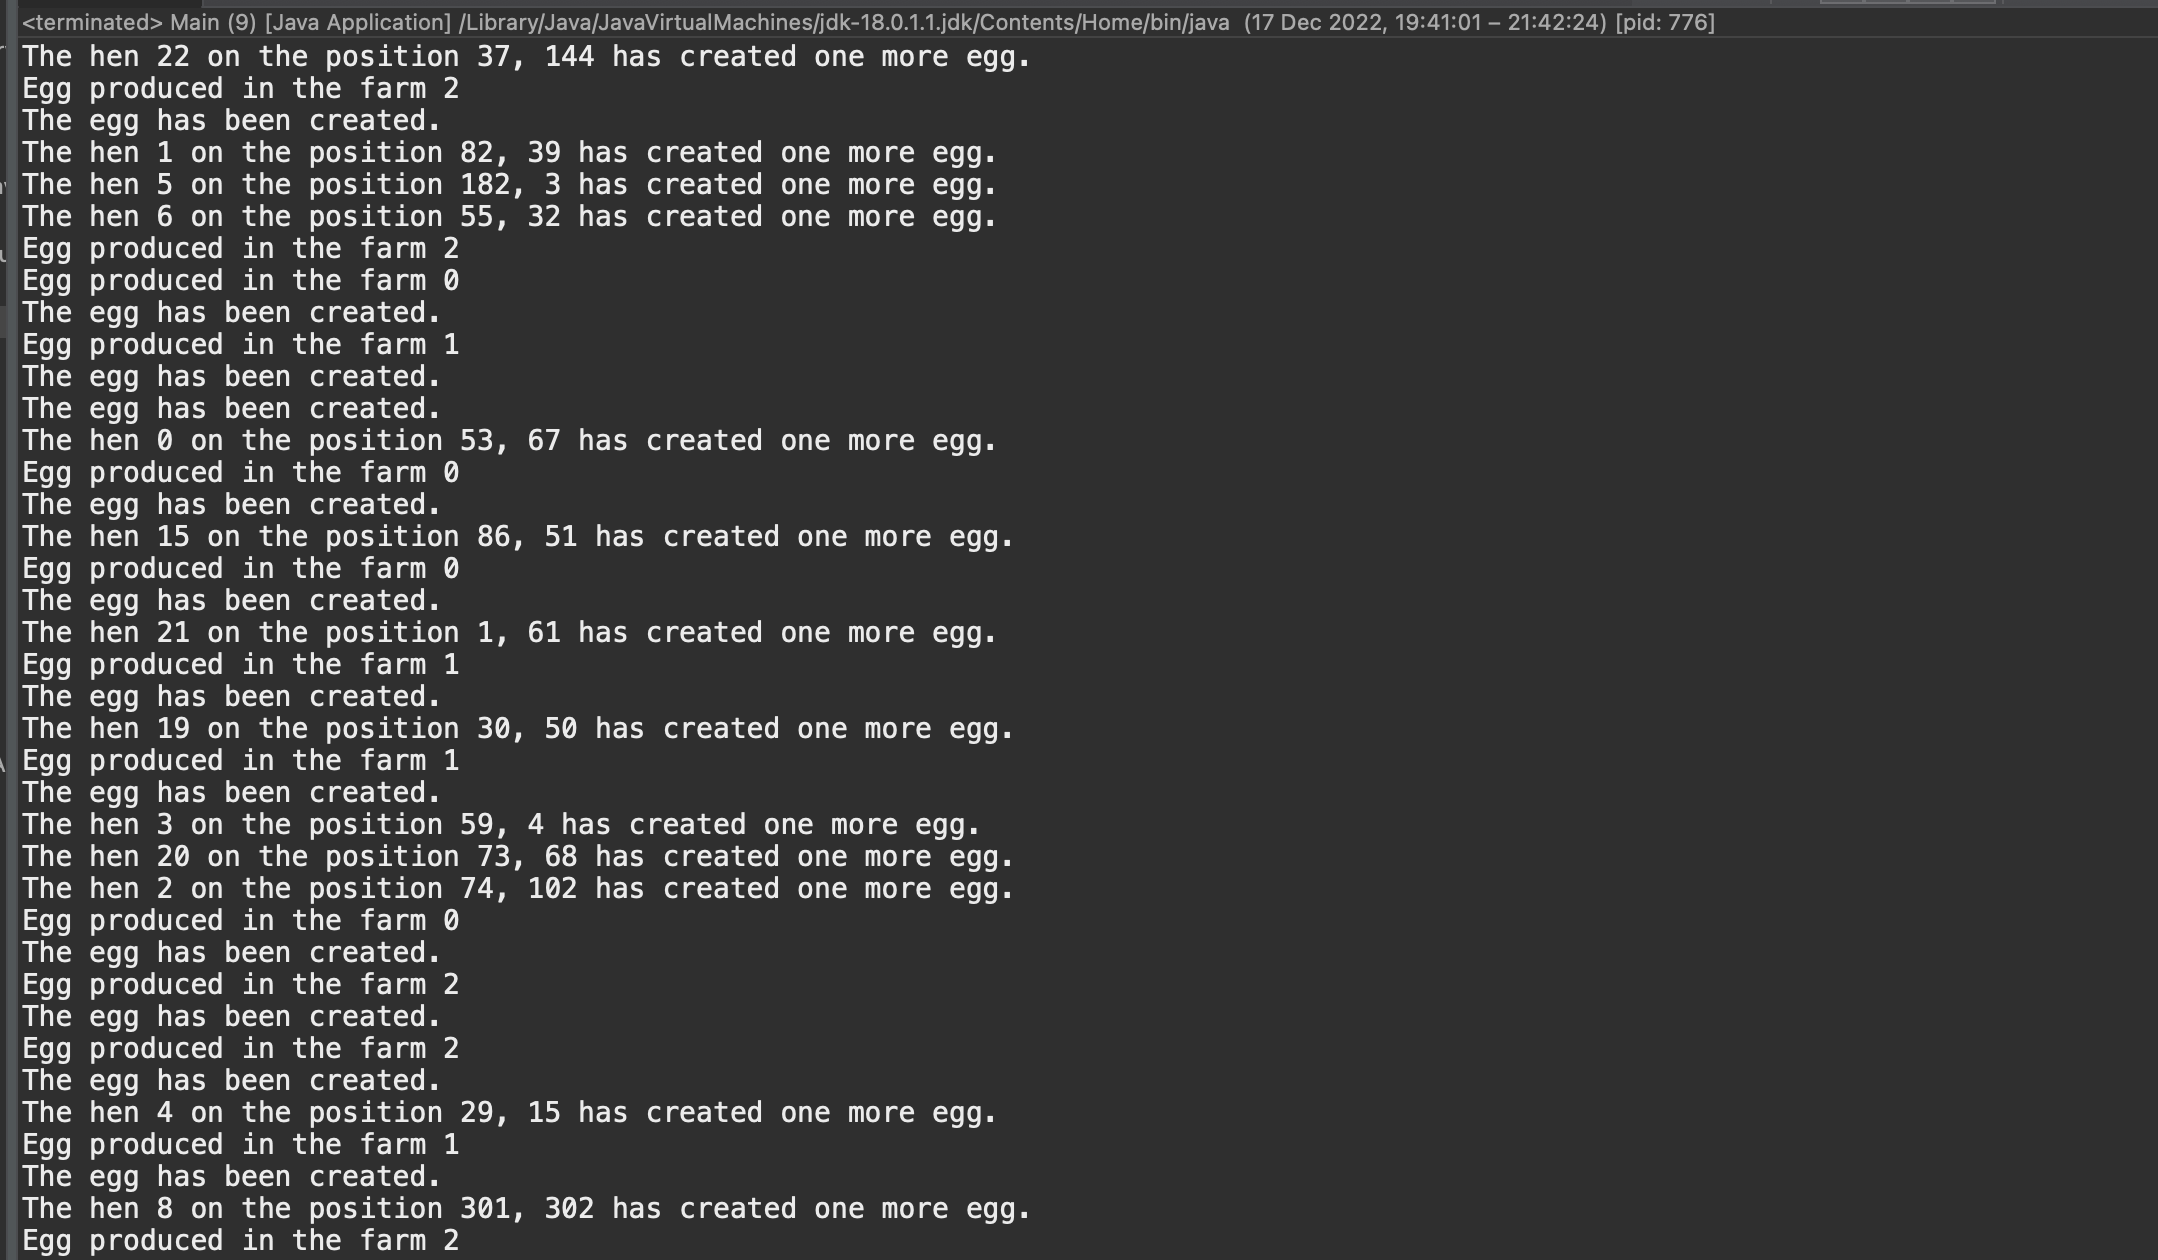
\includegraphics[width=10cm]{Output1.png}
\end{figure}

\begin{figure}[hbp]
    \centering
    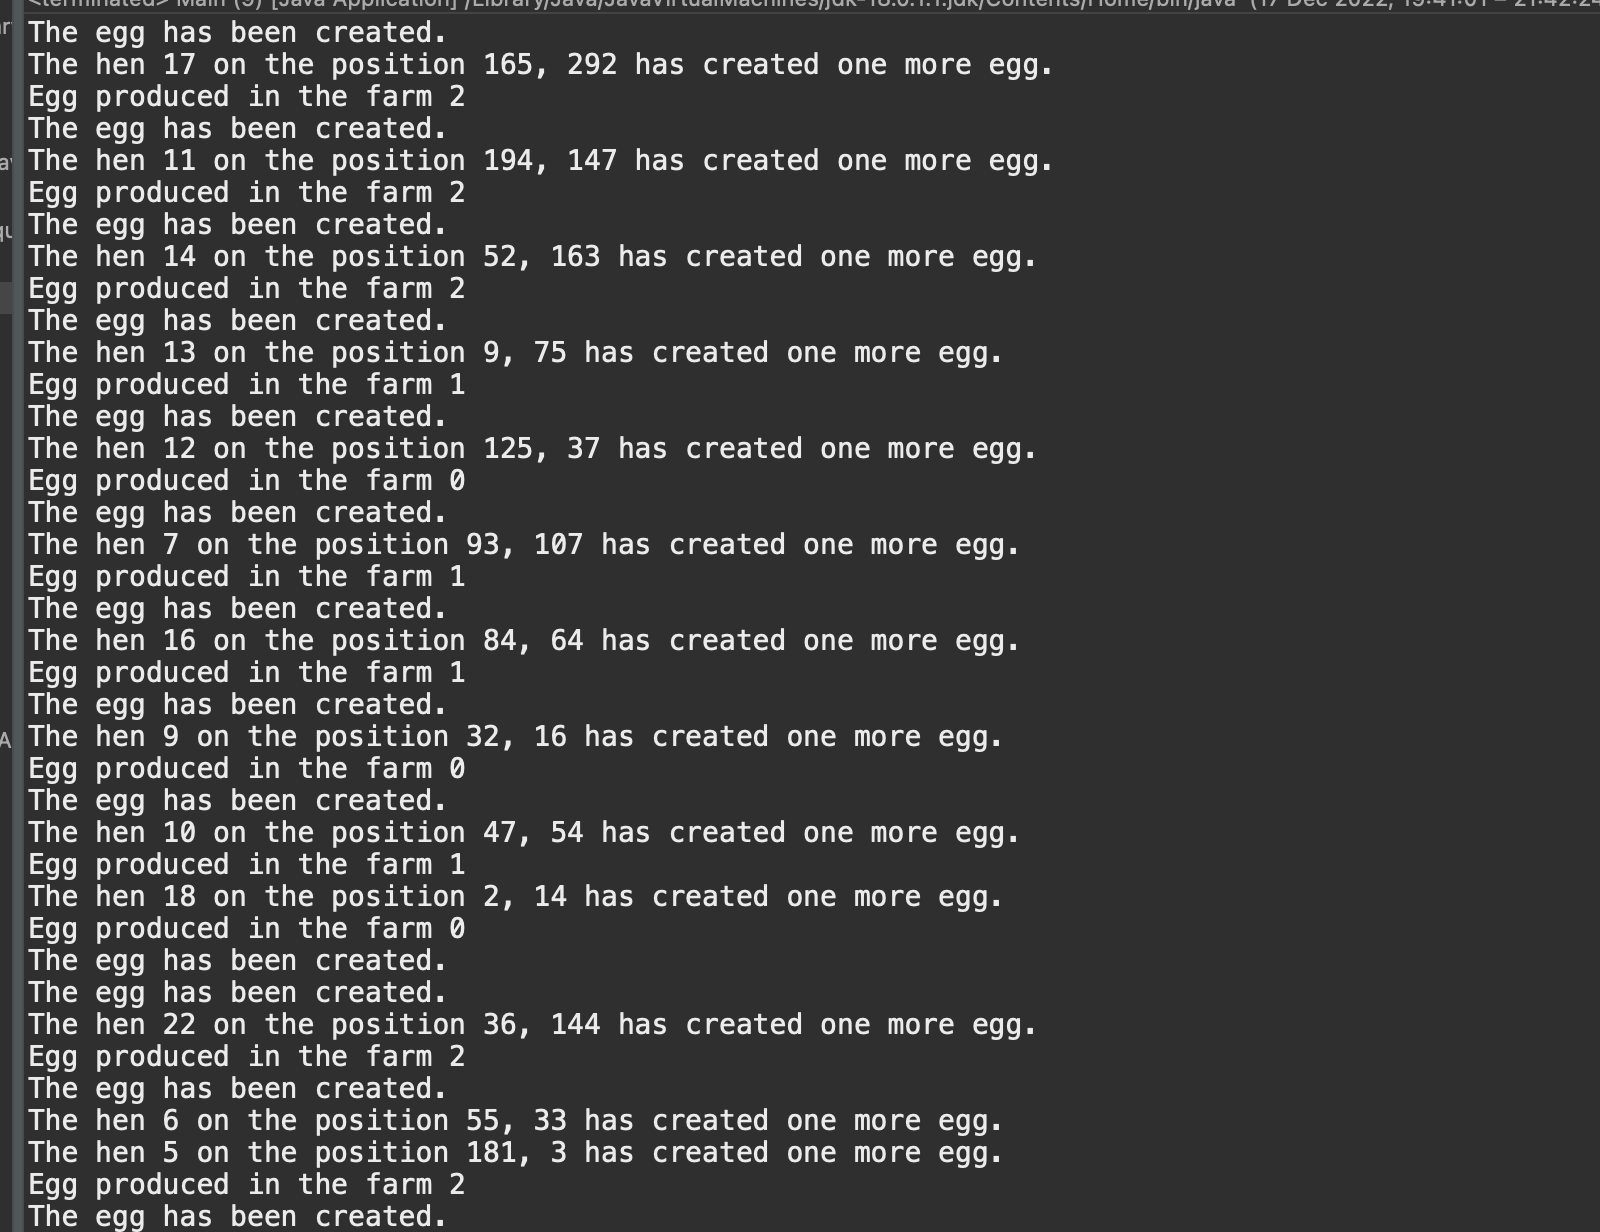
\includegraphics[width=10cm]{Output2.png}
\end{figure}

\begin{figure}[htp]
    \centering
    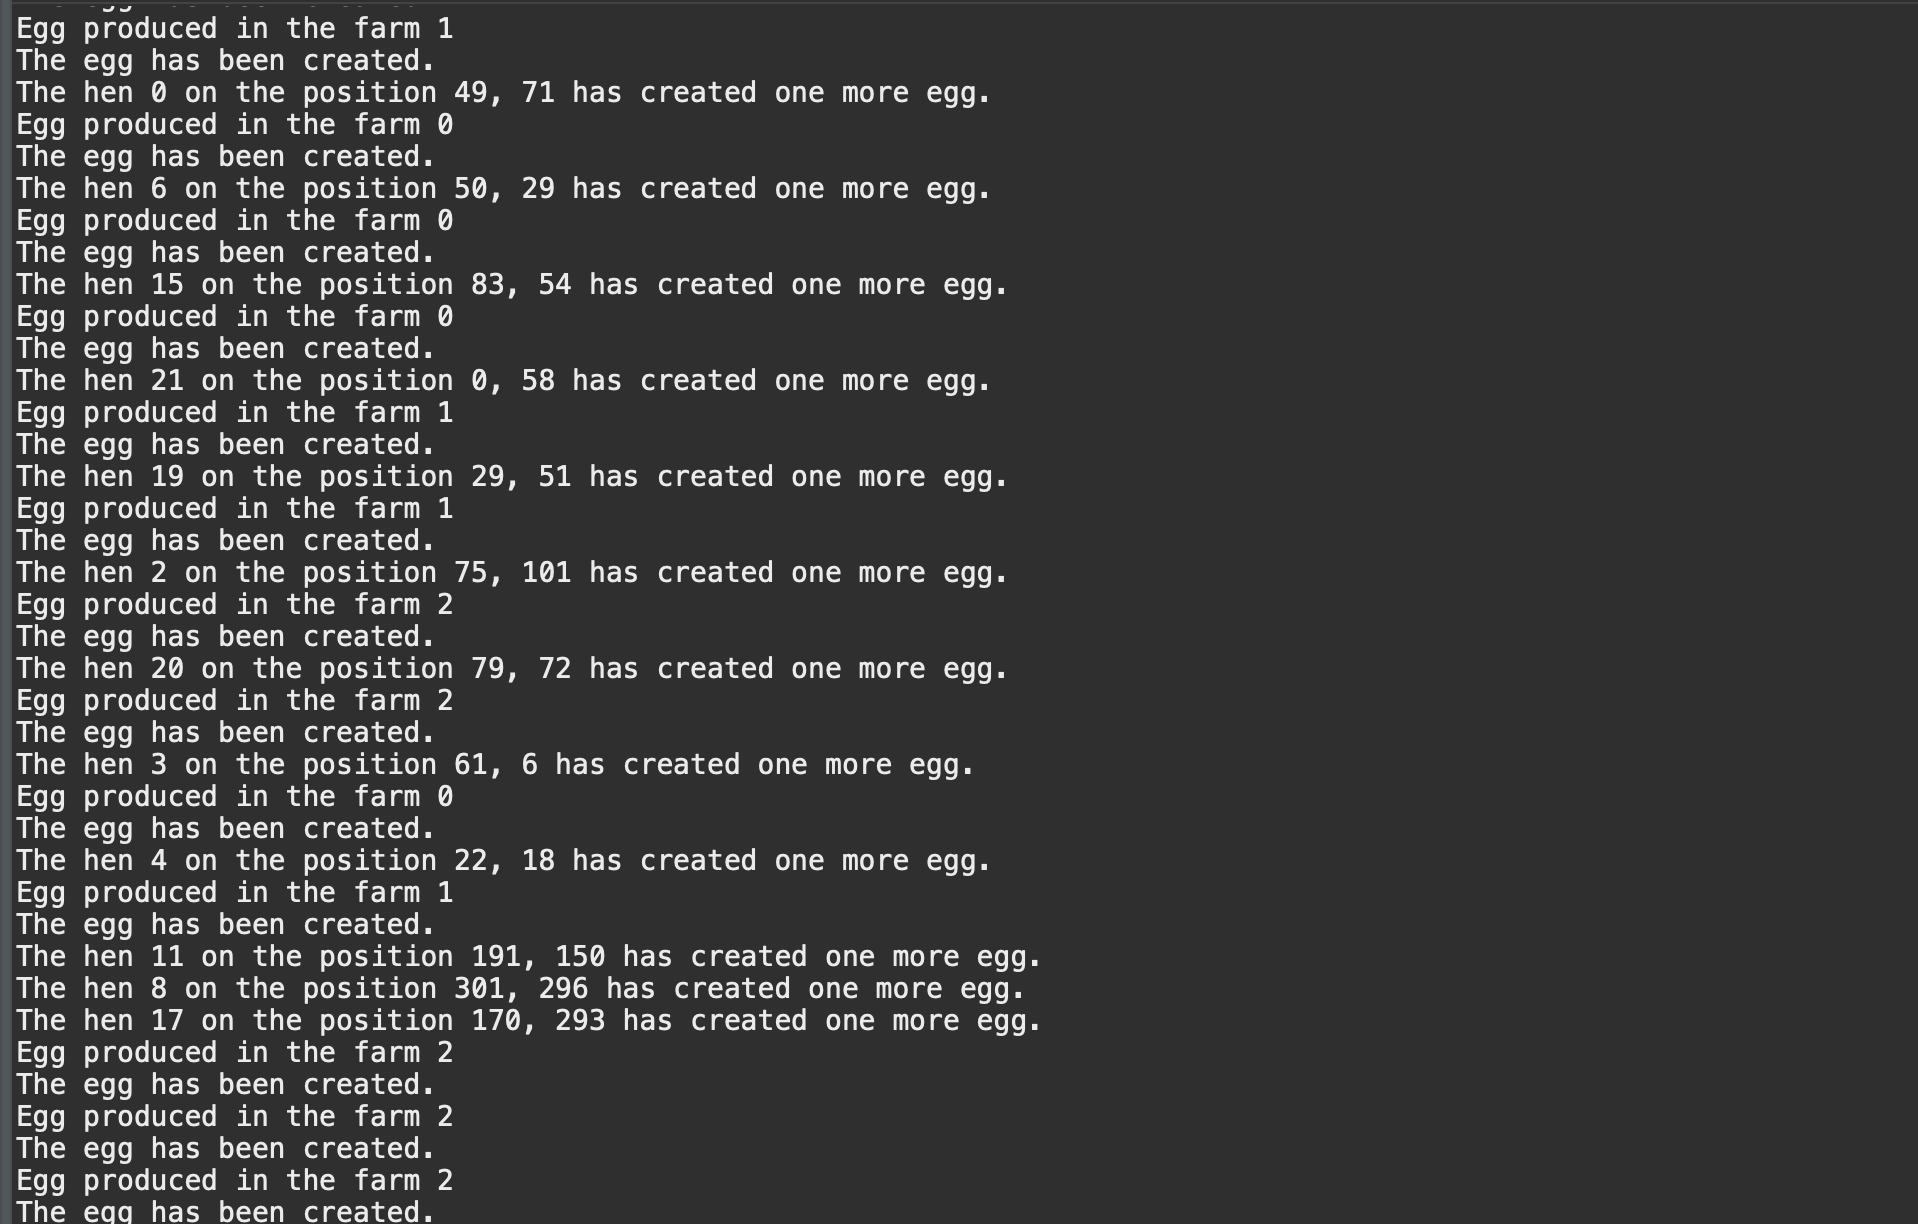
\includegraphics[width=10cm]{Output3.png}
\end{figure}
\newpage
\section{Conclusions}
To conclude, in developing a solution to a problem, it can be quite beneficial to consider the data and the format in which they are presented. It can be a waste of resources (time and memory in the case of computing) to manipulate data that communicates more information than needed to answer a given question. \\
The main purposes of this project are to implement the farm with its given instructions, making use of the prerequisites of  concurrency in Java programming language . After the completion of the assignment, I became familiar with a various  number of features provided by the concurrent interface ( such as semaphores, locks, sockets, synchronized methods etc) and LaTeX. At the same time, I've managed to create a programming work style, which enables me to arrange the source code in a much more readable and organized way.\\
The most challenging part of the project was to move one hen at a  time, as changing a hen's position / an egg's position or an employee who transfers an egg to a farm are actions that cannot be performed simultaneously. For making the right choice, I started by thinking of all the possible solutions and writing a basic approach for each one, until I have found the most efficient one. Therefore,  I have    implemented the moveLock() method. \\
Thus, the structure of the project is composed in such a way
as we can  make sure that an upper object does not terminate, except the case in which all the other objects controlled by it are already terminated. 
\section{References}
[1] Classroom courses and laboratories \newline \newline 
[2] LATEXproject site, http://latex-project.org/, accessed in April 2013. \newline  \newline 
[3] Geeks for geeks site, https://www.geeksforgeeks.org/ \newline \newline 
[4] Stack overflow site, https://stackoverflow.com/  






\end{document} 
